%------------------------------------------------------------------------------
% Template file for the submission of papers to IUCr journals in LaTeX2e
% using the iucr document class
% Copyright 1999-2013 International Union of Crystallography
% Version 1.6 (28 March 2013)
%------------------------------------------------------------------------------

\documentclass[preprint,pdf]{iucr}              % DO NOT DELETE THIS LINE

     %-------------------------------------------------------------------------
     % Information about journal to which submitted
     %-------------------------------------------------------------------------
     \journalcode{J}              % Indicate the journal to which submitted
                                  %   A - Acta Crystallographica Section A
                                  %   B - Acta Crystallographica Section B
                                  %   C - Acta Crystallographica Section C
                                  %   D - Acta Crystallographica Section D
                                  %   E - Acta Crystallographica Section E
                                  %   F - Acta Crystallographica Section F
                                  %   J - Journal of Applied Crystallography
                                  %   M - IUCrJ
                                  %   S - Journal of Synchrotron Radiation
%\usepackage[format=plain,justification=raggedright,singlelinecheck=false,font=small,labelfont=bf,labelsep=space]{caption}
%\usepackage{lineno}
\usepackage[pdftex]{graphicx}
%\usepackage{epstopdf}
\usepackage{float}

\begin{document}                  % DO NOT DELETE THIS LINE

     %-------------------------------------------------------------------------
     % The introductory (header) part of the paper
     %-------------------------------------------------------------------------

     % The title of the paper. Use \shorttitle to indicate an abbreviated title
     % for use in running heads (you will need to uncomment it).

\title{Online data analysis at ESRF bioSaxs beamline}
%\shorttitle{Short Title}

     % Authors' names and addresses. Use \cauthor for the main (contact) author.
     % Use \author for all other authors. Use \aff for authors' affiliations.
     % Use lower-case letters in square brackets to link authors to their
     % affiliations; if there is only one affiliation address, remove the [a].

\author[a]{Martha Elisabeth}{Brennich}
\cauthor[a]{J\'er\^ome}{Kieffer}{jerome.kieffer@esrf.fr}{}
\author[a]{Guillaume}{Bonamis}
\author[a,b]{Alejandro}{De Maria Antolinos}
\author[c]{Stephanie}{Hutin}
\author[a]{Petra}{Pernot}
\author[b,c]{Adam}{Round}
\aff[a]{European Synchrotron Radiation Facility, 71 avenue des Martyrs, CS 40220, 38043 Grenoble \country{France}}
\aff[b]{European Molecular Biology Laboratory, Grenoble Outstation, 71 avenue des Martyrs, CS 90181, 38042 Grenoble \country{France}}
\aff[c]{Unit for Virus Host Cell Interactions, Universit\'e Grenoble
Alpes-EMBL-CNRS, 71 avenue des Martyrs, CS 90181, 38042 Grenoble, \country{France}}

     % Use \shortauthor to indicate an abbreviated author list for use in
     % running heads (you will need to uncomment it).

\shortauthor{Brennich, Kieffer et al.}

     % Use \vita if required to give biographical details (for authors of
     % invited review papers only). Uncomment it.

%\vita{Author's biography}

     % Keywords (required for Journal of Synchrotron Radiation only)
     % Use the \keyword macro for each word or phrase, e.g.
     % \keyword{X-ray diffraction}\keyword{muscle}

\keyword{Online data-analysis, solution scattering, protein}

     % PDB and NDB reference codes for structures referenced in the article and
     % deposited with the Protein Data Bank and Nucleic Acids Database (Acta
     % Crystallographica Section D). Repeat for each separate structure e.g
     % \PDBref[dethiobiotin synthetase]{1byi} \NDBref[d(G$_4$CGC$_4$)]{ad0002}

%\PDBref[optional name]{refcode}
%\NDBref[optional name]{refcode}

\maketitle                        % DO NOT DELETE THIS LINE

\begin{synopsis}
Low-latency SAXS data reduction for bioSAXS and real-time feed-back to the users
\end{synopsis}

\begin{abstract}
High throughput small-angle X-ray scattering on proteins in solution at
synchrotron sources is a commonly used technique in structural biology which
relies on highly automated data acquisition.
Data reduction and primary analysis for bioSAXS experiments consists of a
well-defined series of individual tasks whose automation allows easy first
assessment of the quality of collected data and adjustment of collection strategies if necessary.
This article describes both the logic and the technical implementation of the
automated processing pipeline for bioSAXS data at the ESRF BM29 beamline using
the EDNA framework.
\end{abstract}


\section{Introduction}
The popularity of small-angle X-ray scattering on proteins and nucleic acids in
solution (bioSAXS) to resolve their three-dimensional shape is continuously
growing \cite{Graewert2013,Hura2009,Reyes2014}.
This has not only resulted in the construction of new dedicated
synchrotron beamlines, such as BM29 at ESRF, P12 at EMBL Hamburg or B21 at
Diamond Light Source \cite{BM29paper,P12,B21}, but also pushed forward new
developments in both beamline instrumentation and sample handling.
Examples for this trend are the development of dedicated sample changers
\cite{SCpaper} or the integration of size exclusion chromatography (SEC) systems
into existing beamlines to ensure the mono-dispersity of the sample a a given
time \cite{SECPaper2012,SECP12,SECSWING}.
The \textit{BioSAXS} beamline, BM29, at the synchrotron ESRF, is a small angle
X-ray scattering beamline dedicated to structural biology \cite{BM29paper}.
Currently, the beamline provides two main experimental modes; use of the
bioSAXS sample changer to collect data on alternating buffer\/sample\/buffer
sequences (so called: SC mode) and an online HPLC system \cite{SECPaper2012} for
SEC-SAXS experiments (called HPLC mode).
In both SC and HPLC mode, data are typically collected at a rate of one frame per second
(1 fps).
In order to estimate the quality and usefulness of the acquired data, it is
necessary to process them in a quick and robust way, compatible with the
throughput of the beamline.

Available processing tools for SAXS data which support online processing of
large data sets include \textit{DPDAK} \cite{DPDAK}, \textit{bioXTAS raw}
\cite{BioXTASraw}, \textit{SAXSutilities} \cite{SAXSUtilities} and
\textit{SASFLOW} \cite{X33P,P12},  \textit{XRDUA} \cite{xrdua}, \ldots
Most of these either require some advanced input from users or are not open source.
An alternative to these dedicated SAXS tools are more general open source frameworks such as
\textit{EDNA} which is for example used for macromolecular crystallography at
ESRF \cite{EDNA}.
Our goal was to develop a robust set of online auto-processing pipelines
for bioSAXS experiments, including data reduction, primary analysis and
\textit{ab-initio} modeling  within the EDNA framework.
The additional needs for flexibility and minimization of
direct user interaction, led us to develop pipelines for both SC and HPLC mode with EDNA.
These pipelines use pyFAI for azimuthal integration \cite{pyFAI} and tools
from the \textsc{atsas} package \cite{ATSAS1,ATSAS2} for analysis and modeling.
Some parts of the \textsc{atsas} package have been re-implemented as a Python
library (named FreeSAS \cite{freesas}) for a better integration into the
Python-based pipeline.
All data analysis is smoothly integrated with the beamline control system
(BsxCuBe) and the ISPyBB \cite{ISPYBB} database.


Online data analysis is a key component of any highly automated beamlines
where the acquisition of a sample lasts a few seconds and without dead-time between samples.
Therefore the processing speed must at least keep up with the data acquisition, which
at ESRF-BM29 is typically one frame per second and about three minutes for a set
of background and sample measurements in sample changer mode.


\subsection{Experiment control}
Data acquisition at the ESRF-BM29 beamline is controlled via the BsxCuBe
graphical interface, written in Python/Qt4 \cite{pyqt}.
BsxCuBe is composed of control-objects which communicate with other beamline
components (i.e. detector, motors, sample changer, data analysis server\ldots)
via the tango protocol\cite{tango}.

%\subsection{Data analysis server}

%Data analysis is triggered automatically by BsxCube via a tango call.
%The data analysis server is actually a tango device server written in
%PyTango\cite{pytango} which launches EDNA jobs \cite{edna}.


\subsection{EDNA}
EDNA \cite{EDNA} is a plugin-based framework to build pipelines for data-analysis.
The basic idea behind EDNA is to have plugins which are either responsible for the execution
of a task or an external process (called \textit{execution plugins}) or in
charge of launching and managing other plugins, either sequentially or in
parallel (called \textit{control plugins}).
The number of execution plugins running simultaneously is limited by processor
resources of the computer (and the Python global interpreter lock).
Any plugin receives its input arguments and returns its result using
EDNA data-structures (actually Python objects) which can be serialized into XML
for saving on the disk or sending them over the network.

An EDNA job is a top level control plugin which communicates with the outside
world, providing its state, or its results even after processing is finished,
while keeping its memory footprint as small as possible.

\subsection{The Tango device server}
For accepting processing jobs from the outside, e.g. from the data
acquisition software (BsxCuBe), EDNA provides a Python based Tango device
server interface \cite{tango,pytango}.
The device server starts EDNA jobs via the \textit{startJob} command.
The parameters of this command are a plugin name and the input data-structure
associated with it (serialized); and returns a job identifier to the requester.
This Tango device server is hence completely generic and can be used for any
type of EDNA jobs.

To achieve maximum responsiveness at the Tango level, EDNA jobs are not started as
they arrive but they are just instantiated and queued.
Another thread is responsible for starting them and can start multiple jobs in parallel
(data-parallelism).
The number of jobs and the number of actual execution
plugins running simultaneously is controlled independently to make the best use
of the computing resources available.

Once finished, every EDNA job emits a tango-event to announce the results are
available with its status: success or failure.
Other processes, e.g. the data acquisition software, can then retrieve the result
of the processing, e.g. the 1D integrated scattering curve and
display it without reading from the disk.
This architecture allows to start processing for individual images or to
display curves instantaneously without polling the shared file-system.
This improves greatly the responsiveness as synchronization of shared
file-systems across the network often exhibits delays of multiple seconds.

\subsection{Hardware, software and versions}
Two computers with GP-GPU computing capabilities (Nvidia Quadro 4000) are
dedicated for online data analysis on the \textit{bioSAXS} beamline BM29, they are
independent and feature the same software installation.
As the \textit{ab-initio} reconstruction pipeline lasts of dozens of minutes
(due to the final refinement stage using \textit{dammin}), it is run on the most
powerful computer whereas the azimuthal integration pipeline, which needs the lowest
latency, is run on the smaller computer.
A third computer with similar computing capabilities is available for
\textit{off-line} reprocessing, development of pipelines and acts as a spare.
All three computers are running Debian 7 operating system with \textsc{atsas}
(version 2.6.1).



\section{Data analysis pipeline in sample changer mode}

Using the sample changer allows a high throughput of different samples (
$\sim 3$~min/sample).
Before and after measuring a sample, a background measurement using its
corresponding buffer is performed.
If the buffer of a sample is the same as the one of the preceding sample, the
background measurement before the sample is dropped, as it is identical to the
buffer measurement after the preceding sample.
Hence, data is produced in sequences of the type \textit{buffer 1, sample 1,
buffer 1, buffer 2, sample 2, buffer 2, \ldots}  or  \textit{buffer 1, sample 1,
buffer 1,  sample 2, buffer 1 \ldots}.
Typically for each buffer or sample, 10 frames of 1~s exposure time are acquired.

The following steps for data reduction and analysis are required:
\begin{enumerate}
\item the azimuthal integration of an individual frame,
\item the creation of a background corrected sample curve,
\item basic analysis of the sample curve (Guinier plots, and other invariants)
\item \textit{ab-initio} modeling based on the basic analysis.
\end{enumerate}
In the EDNA bioSAXS application (2) and (3) are combined into one pipeline.

\subsection{Azimuthal integration pipeline}
\label{AI}
The azimuthal integration pipeline is triggered for every single frame acquired, i.e. every second,
and therefore needs to have the lowest latency possible to display the integrated curve
in \textit{real time} in the graphical beamline control interface BsxCuBe.
The input data-structure for azimuthal integration contains
information about the geometry of the experiment, the sample, its concentration
and the transmitted intensity (I1) as measured on the beam-stop diode for
normalization, etc.
To cope with the requested speed (up to 10 frames per second), this pipeline
has been optimized and simplified to the maximum.
It relies on the FabIO \cite{fabio} package for image reading (from NFS-mounted
disks) and pyFAI \cite{pyFAI} for azimuthal integration.
As the images are acquired with a Pilatus 1M pixel detector (from Dectris), the
error can be assumed to be Poissonian and is integrated as such.
The azimuthal integration calculation is performed on a dedicated graphics card
(Nvidia Quadro 4000) using OpenCL \cite{pyFAI_gpu}, offloading this processing
from CPU to GPU, hence leaving resources to other pipelines.
Subsequent normalization are performed directly using NumPy~\cite{numpy}.
The result is saved into a 3-column ASCII file suitable for further processing
using the \textsc{atsas} tools \cite{ATSAS2} and sent back to BsxCuBe for
live display.
In accordance with EMBL and ESRF standards, the scattering vector
$q=4\pi\frac{\sin(\theta)}{\lambda}$ is given in inverse nanometers.

\subsection{Curve merging, background correction and basic analysis}
\label{SM}
Data acquisition is usually performed  in sets of sample and buffer measurements.
Each sample or background measurement consists of set of frames
(typically 10) in order to be able to detect radiation damage
(preventing the interpretation of data from damaged samples).
The \textit{SmartMerge} pipeline is triggered at the end of each measurement
and is responsible for evaluating the similarity of different scattering
patterns, using the \textit{datcmp} tool from \textsc{atsas} and merging all frames
similar to the first and propagate the associated meta data and errors.
A flow diagram is provided in figure~\ref{fgr:smart}.
All curve comparisons can be performed in parallel on modern multicore
computers thanks to EDNA multi-threaded environment.
Subsequently, the \textit{SmartMerge} plugin averages the individual frames
of a measurement, controls for the buffer-sample-buffer sequence and
 calls the \textit{autoSub} plugin, which determines the optimal buffer
(see hereafter) and subtracts it from the sample data,  providing the 
\textit{subtracted curve} containing only the scattering from the macromolecule
of interest.
If the buffers measured before and after the sample are considered sufficiently
similar by \textit{datcmp} ($p > 0.01$), the optimal buffer is their average.
If they differ too much ($p \leq 0.01$), each of them is subtracted individually from the
sample curve and the difference which results in  the smallest radius of gyration ($R_{G}$),
as determined by the tool \textit{autorg} from \textsc{atsas}, is retained.
If both values of $R_{G}$ are identical, the selection is made using the lowest forward scattering intensity $I_{0}$.
If \textit{autorg} fails for both subtracted curves, the buffer with the lowest total scattering is selected.
Figure~\ref{fgr:autosub} provides a flow chart of the plugin.

Finally this \textit{subtracted curve} is analyzed using the
\textit{SaxsAnalysis} plugin which performs subsequently applies tools from the \textsc{atsas} package for Guinier region fitting
using \textit{autorg}, inverse Fourier transform using \textit{datgnom} to obtain
$p(r)$ and Porod volume assessment using \textit{datprorod}.
In addition the \textit{SaxsAnalysis} plugin creates \textit{PNG} figures of
the subtracted curve and the fit created by \textit{datgnom}, the Guinier fit,
the $p(r)$ function and Kratky plots whenever possible (Figure~\ref{plots}).
All these information and figures are then directly returned to BsxCuBe to inform the user
of the success of the experiment and additionally logged into the ISPyBB
database \cite{ISPYBB} where they can be accessed via an web interface.
Figure~\ref{fgr:analysis} provides a flow chart of the plugin.

\subsection{Ab-initio reconstruction pipeline}
\label{abinitio}
Following the analysis, a three dimensional, dummy atom model based
on the \textit{subtracted curve} is reconstructed.
This pipeline is inspired from a preliminary work
performed at the Diamond Light Source \cite{DiamondSE}.

It runs multiple instances of \textit{dammif} in parallel (8 or 16 by default)
to get multiple models \cite{dammif}, taking benefit of the multi-threading
environment of EDNA.
Multiple models are created in order to give a visual indication of the variation in
reconstruction and to avoid over-interpretation and biased decisions based on
the models.
After a first round of outlier rejection based on the goodness of fit ($R_{f}$)
and the $\chi^{2}$ where the threshold is the mean plus two standard
deviations, only $N$ valid models remain.

All $N$ remaining models are superimposed two by two using
our open source implementation of \textit{supcomb}, supycomb, which is available freely
(MIT license) as part of the FreeSAS package \cite{freesas}.
Former versions of the pipeline have been using the original
\textit{supcomb} \cite{supcomb} program from \textsc{atsas} by launching
$N*(N-1)/2$ processes in parallel within the EDNA framework.
It turned out to be more advantageous (in term of speed) to read all models
from disk only once and perform the all alignment in memory.
The distance calculation (actually normalized spatial discrepancy, NSD) has
been optimized using a binary extension (Cython parallel code).
All other transformations rely on NumPy \cite{numpy} code and the geometric
optimization is performed using the simplex minimizer provided by SciPy \cite{scipy}.

The table containing the NSD is then generated
(Figure \ref{fgr:nsd}), explaining which model is the nearest from all other
valid models. This model is called the reference model and all other valid
models are re-oriented and aligned on the reference one.
All models with an NSD higher than the mean plus one standard deviation are
discarded.

All valid models are merged using \textit{damaver} \cite{damaver}, \textit{damstart} and
\textit{damfilt} and finally refined using \textit{dammin} \cite{dammin}.
This last step is pretty slow an lasts usually for dozens of minutes. 
If it lasts longer then half an hour, we assume that \textit{dammin} will not finish and 
EDNA aborts the process in order to free resources. 
All results are uploaded to the ISPyBB database where they can also be
visualized. Figure~\ref{fgr:modeling} provides a flow chart of the plugin.


\section{Data analysis pipeline in HPLC mode}
While the sample changer allows a high throughput of samples, it requires
homogeneous samples which do not degrade.
Protein samples often are intrinsically heterogeneous.
For example, constituents of a complex might be present in excess or proteins
might aggregate.
One approach to address this issue is to purify the sample directly online by collecting data
on the eluent from a size exclusion chromatography column (SEC-SAXS or HPLC mode) \cite{SECPaper2012,SECP12,SECSWING}.
At the bioSAXS beamline (BM29) we continuously collect 2D-diffraction frames
throughout the SEC purification run at a rate of 0.5 to 5 Hz
(depending on the synchrotron filling mode and the duration of the SEC purification, 1 Hz being the standard),
resulting in up to a few thousand frames.
While we know that the first few frames are acquired on buffer, the sample composition
for later frames is not known \textit{a priori}.
The result of a SEC-SAXS experiment can be very complex.
Our automatic analysis provides data reduction and basic analysis for every
individual frame.
In addition, it uses this information to try to identify regions in the
chromatogram which correspond to one species and merges frames from these
regions to improve the signal to noise ratio.
The goal of this procedure is not to produce an idealized curve of an individual
species but to give a hint on the overall data quality as soon as possible.

\subsection{HPLC single frame pipeline}

The HPLC single frame processing pipeline is triggered for every frame in HPLC mode.
It integrates each frame using the azimuthal integration pipeline (see
\ref{AI}) and compares the result to the first frame using \textit{datcmp} from the
\textsc{atsas} package.
The frame is then classified as buffer, sample, or ``in between''
($p>0.1$, $0.01 > p$, $0.01>p>0.1$  respectively).
The first time a frame in a HPLC run is not classified as buffer, all previous
frames are averaged to yield an ``average buffer''.
For any frame classified as sample, the ``average buffer'' is subtracted, Guinier
analysis is performed (with \textit{autorg} from the \textsc{atsas} package),
providing a radius of gyration $R_G$ and the forward scattering intensity $I_0$,
and the correlated volume is calculated in order to estimate the mass
\cite{RamboTainerNature2013}.
In addition, the plugin also calculates the total scattering intensity of any
frame, regardless of its classification.
This plugin (on the current hardware) can operate at about 2 Hz, but often the
acquisition speed is 1 frame per second, so that the image can be integrated and
displayed in almost real time.



\subsection{HPLC run processing}
When the HPLC experiment ends (or is aborted) a specific plugin (\textit{HPLCflush}) is launched to
finish the processing of the experiment as one SEC-SAXS run.
The plugin uses the results of \textit{autorg} to locate peaks using continuous
wave transformation as implemented in SciPy on the forward scattering
\cite{cwt,scipy}, and then merges all individual curves around a local maxima
of the forward scattering with similar radius of gyration.
All processing results from the \textit{HPLC single frame pipeline} and the results of
the peak finding are saved into a single HDF5 file which is uploaded to the
ISPyBB database at the end of the processing.
In addition, the plugin creates figures (in PNG and in SVG format) of the
total scattering, forward scattering and radius of gyration \textit{vs.} frame
number (or time).
Figure \ref{fgr:SEC} shows the result of an HPLC
experiment where one main peak and a trailing shoulder is identified.
All merged files are further analyzed by the \textit{SAXS analysis}
(\ref{SM}) and the \textit{ab-initio reconstruction pipeline}
(\ref{abinitio}) plugins described for the sample changer pipeline.

\section{Offline data analysis}
In case offline processing is required, e.g. when one of the parameters for
the azimuthal integration of previously processed data needs to be adjusted,
several Python scripts for starting sub-pipelines are available.
Those tools are part of the EDNA installation and just instantiate the needed
plugin and run it with the parameter description file which has been modified
accordingly.
For HPLC mode and curve-merging, there are specific tools to reprocess complete
datasets if needed.

The drawback of this approach is that it relies on the EDNA infrastructure, which is
non trivial to install and even more difficult to customize (path of the
\textsc{atsas} executable and licensing issue, number of cores, GPU
configuration, timeouts for any part of pipelines, \ldots).
The availability of a spare computer on the beamline dedicated for offline
processing removes this need, hence reprocessing never interferes with ongoing
acquisitions.

\section{Practical example}
To illustrate the functionality of the processing pipeline we acquired data collected
on a deletion construct of the protein D5 from  Vaccinia virus (VACV).
Data were acquired as both a dilution series using the sample changer as well as
using SEC-SAXS (see figures \ref{fgr:SCcurves}, \ref{fgr:SEC} and \ref{fgr:curves} respectively).
The online analysis results of the sample changer data indicate concentration effects
as the radius of gyration decreases with the  sample concentration (see table~\ref{tbl:results}).
To eliminate potential undesired oligomers (e.g. aggregates), we additionally performed a SEC-SAXS run.
The total scattering chromatogram provided nearly instantaneously via BsxCuBe displays a strong main
peak with extended tails both sides (see figure \ref{fgr:SEC}).
After the completion of the run, the complete analysis results can be examined via
ISPyBB.
The forward scattering intensity shows the same peak as the total scattering intensity.
In the early frames of the peaks both the radius of gyration and the mass estimate get systematically
smaller with higher frame number, indicating a larger component.
Both stabilize with higher frame numbers and stay stable until the end.
The auto-processing chose the region underlined blue in figure  \ref{fgr:SEC}
for merging the data.
For further manual processing and modeling of the protein, we chose the smaller
striped region.
Direct comparison of the two merged curves that they only differ in the noise level
(see figure \ref{fgr:curves}).
Comparison of the radius of gyration of the SEC-SAXS data with the data acquired with the sample
changer shows a consistently lower radius of gyration (see table \ref{tbl:results}), and direct
comparison of the curves shows a slightly higher signal at low angles for sample changer data,
indicating aggregates.

%In our example, the auto-processing helped us to optimize our experiment on the fly.

\section{Conclusions and Outlook}
As illustrated by our example, auto processing has become an invaluable tool for
experiments at the \textit{bioSaxs} beamline BM29, enabling optimization of the
data acquisition parameters to obtain the best data, avoiding the effects of
radiation damage on the data, measuring additional dilutions where inter-particle 
scattering is observed or switching to online SEC where necessary, \ldots 
Additionally where data quality is good the feedback allows efficient use of
beamtime avoiding additional unnecessary measurements and giving users confidence 
to move to the next highest priority samples.
The combination of the auto processing results being available and their presentation 
in a user friendly manner in ISPyB facilitates experiments for both experienced users 
by enabling them to spend more time preparing samples and acquiring data 
(instead of data processing), and for newcomers to the beamline and technique 
to whom  the software tools and their use might be unfamiliar. 
Auto processing gives the users real time feedback on data quality and the progress 
of the experiment enabling them to spend more time thinking about their science and 
how to do the best experiment.
Additionally the automation of data processing along with data acquisition, an
efficient experiment and thorough experiment can be confidently carried out by an individual.

To enhance further the user experiment, the delay of feed-back to the user
should be kept minimal, providing systematically a consistent result.
For now, the weakest point of all processing pipelines is the
\textit{ab-initio} modeling pipeline which may have aborted the
execution of the \textit{dammin} process (often due to a time-out in
the EDNA plugin: the sub-process did not quit as requested).
By re-implementing this Monte-Carlo modelling step in parallel into FreeSAS, it
could be integrated directly into the EDNA pipeline and maintain the execution
time within a couple of minutes, providing faster feed-back to the user.

%The modularity of the EDNA-plugin based approach facilitates the addition of
%new tools as well as the re-use of existing plugins for other purposes. For
%example, it will be easy to add new tools such as \textsc{shanum}
%\cite{SHANUM}, which estimates the number of meaningful Shannon channels,
%without affecting the integrity of the existing pipline.
%Additionally, the existing EDNA plugins can easily be integrated into more
%complex workflows such as those already available for macromolecular
%crystallography \cite{workflow}.

\appendix
\ack{The authors would like to thank Ricardo Fernandes and Thomas Boeglin for developing
the original offline reprocessing tools, Peter Boesecke for the original azimuthal
integration procedure, Olof Svensson for the development of EDNA, Irakli Sikharulidze for
the original version of the \textit{ab-initio} modeling pipeline,
Alexey Kikhney, Daniel Franke and Dmitry Svergun for the \textsc{atsas} package and support
in its implementation, Staffan Ohlsson and Matias Guijarro for integration with the data
acquisition software, Wim Burmeister for helpful discussions and support, Claudio Ferrero,
head of data analysis unit, for the critical revision of this
manuscript.
Stephanie Hutin was supported by an ANR grant (REPLIPOX, ANR-13-BSV8-0014).}


\bibliographystyle{iucr}
\bibliography{biblio}


\section{Preparation of protein sample and data acquisition}
All examples of protein data in this manuscript are based on a deletion construct of
the D5 protein from vaccinia virus (VACV).
The sequences of D5R is from the VACV strain Copenhagen (GenBank accession number M35027.1).
D5 391-785 was cloned into the pProEx Htb plasmid (Invitrogen), fused to an N-terminal
TEV(tobacco etch virus) protease-cleavable hexahistidine tag. The protein was expressed in
BL21* and purified over a HIS-select column (Sigma) (lysis buffer: 50 mM Tris pH 8.5, 150 mM NaCl,
5 mM MgCl$_{2}$, Complete protease inhibitor cocktail (Roche), DNaseA, 10 mM beta-Mercaptoethanol; 
binding buffer: 50 mM Tris pH 8.5, 150 mM NaCl, 10 mM beta-Mercaptoethanol; 
high salt wash buffer: 50 mM Tris pH 8.5, 1 M NaCl, 10 mM beta-Mercaptoethanol, 
elution buffer: 50 mM Tris pH 8.5, 150 mM NaCl,  200 mM imidazole, 10 mM beta-Mercaptoethanol). 
The buffer of the eluates was exchanged to binding buffer on a PD10 column and the protein was 
TEV-digested over night at RT. After a second Ni-column, the sample was injected onto a 
Superdex 200 GL 10/300 column (GE Healthcare) equilibrated with gel filtration buffer 
(20 mM Tris pH 8.5, 150 mM NaCl, 1 mM dithiothreitol (DTT)). Eluted peaks were analyzed by 
SDS-PAGE, stained with InstantBlue (Expedeon).
For sample changer mode a dilution series of five different concentrations was prepared
(see table~\ref{tbl:results}). For size exclusion we injected 50~$\mu$l of sample at 20~mg/ml on a Superdex
200 5/150 GL column (GE healthcare).


\section{Software distribution and licensing}

All software developed for online data analysis at the bioSAXS beamline is
open-source.
Nevertheless it relies on the \textsc{atsas} package which, while free for
academic use, is neither open-source, nor redistributable.

EDNA is licensed under LGPL for the kernel part (the pipeline engine) and GPL
for the bioSAXS part. The source code is now hosted on a public
repository at:\\https://github.com/edna-site.
While open-source, EDNA is a
server tool for online data analysis and the developers are aware how difficult
it may be to install and configure it properly. EDNA is controlling
\textsc{atsas} modules by executing external programs in pipe-mode to avoid any
licensing issues.

The azimuthal integration is performed via pyFAI \cite{pyFAI}, the Python library
for fast azimuthal integration, which is accelerated on GPU \cite{pyFAI_2015}.
Diffraction image reading is performed by FabIO \cite{fabio}.
Both libraries
are licensed under GPL and hosted under those web pages:\\
http://github.com/pyFAI and https://fable.sf.net
Some \textsc{atsas} parts have been re-implemented in Python to offer a better
integration into the processing pipelines (by avoiding the forking of many
sub-processes): \textit{dataver}, \textit{datop}, \ldots  and
\textit{supcomb} which is available as part of the \textsc{FreeSAS} package
which re-implements the algorithms in a MIT type license. FreeSAS is available
on github at https://github.com/kif/freesas but without guaranteeing any
numerical equivalence with the reference implementation.

Finally the other tools of the Python scientific stack (Numpy, scipy,
matplotlib) are licensed under BSD license.


\begin{figure}
\centering
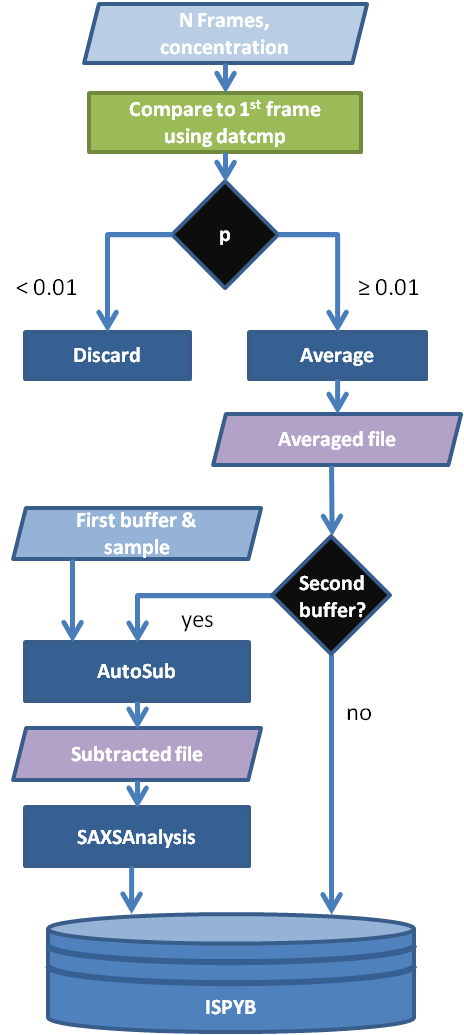
\includegraphics[width=8cm]{smartmerge.png}%
\caption{Flow diagramm of the \textit{SmartMerge} plugin for data reduction.
This plugin controls the averaring of individual frames and launches
subtraction and primary analysis if required.
Light blue parallelograms indicated data input, violet parallelograms data output,
black diamonds decision, green rectangles processing using \textsc{atsas} tools
and blue rectangles processing using non-\textsc{atsas} tools. }
\label{fgr:smart}
\end{figure}

\begin{figure}
\centering
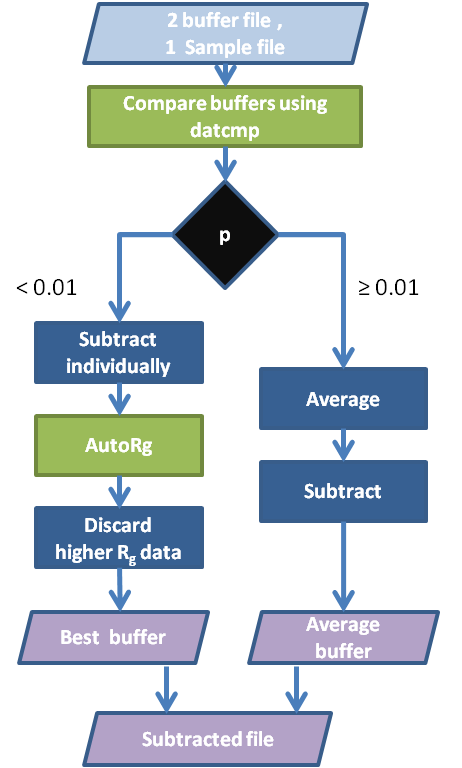
\includegraphics[width=8cm]{autosub.png}%
\caption{Flow diagramm of the \textit{autoSub} plugin for subtracting the best
buffer.
This plugin performs the subraction of the background after choosing the most suited one.
Symbols as described in figure \ref{fgr:smart}.}
\label{fgr:autosub}
\end{figure}

\begin{figure}
\centering
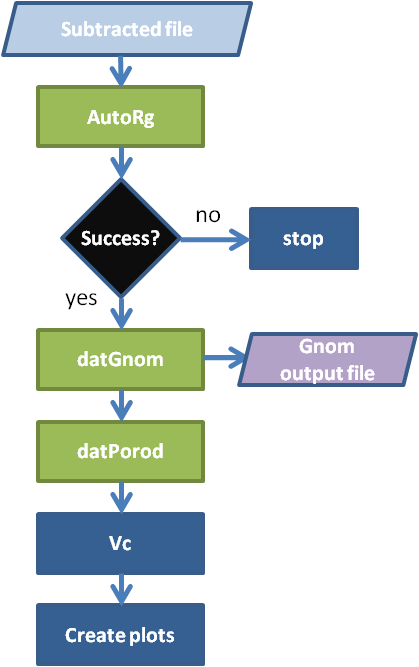
\includegraphics[width=8cm]{analysis.png}%
\caption{Flow diagramm of the \textit{saxsAnalysis} plugin.
This plugin performs various primary analysis methods on background corrected data.
Symbols as described in figure \ref{fgr:smart}.}
\label{fgr:analysis}
\end{figure}

\begin{figure}
\centering
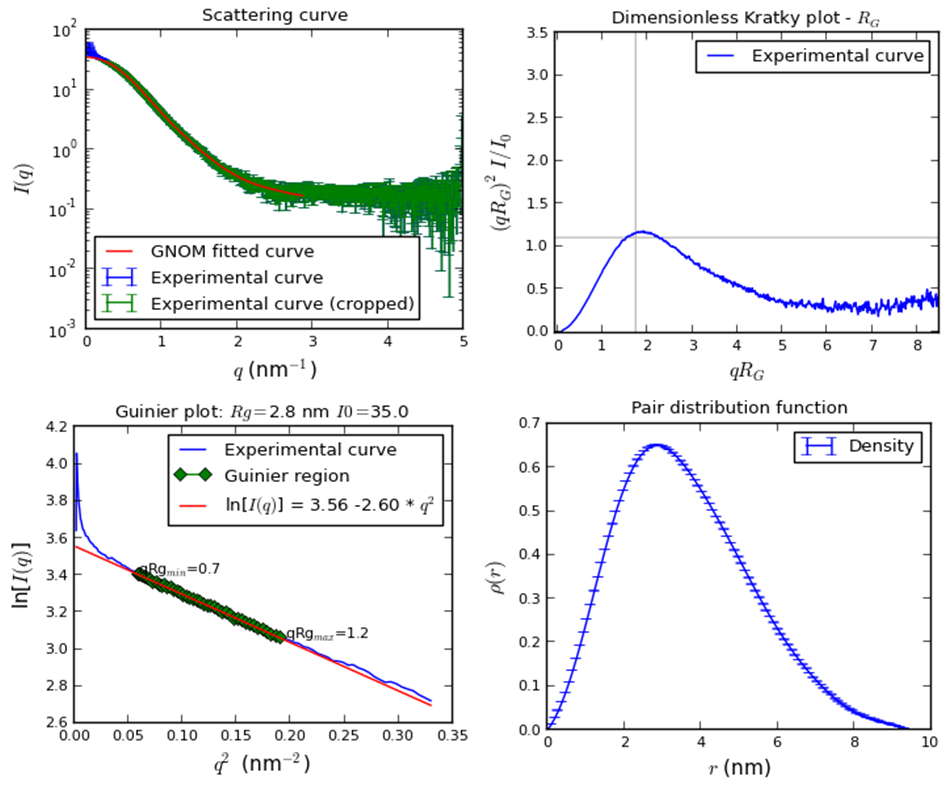
\includegraphics[width=18cm]{autoplot.png}
\caption{Examples of the figures automatically generated by the
\textit{SaxsAnalysis} pipeline: scattering curve, normalized Krakty plot, Guinier plot and pair distribution function.
The layout is adjusted from the standard version for improved readability in
print.}
\label{plots}
\end{figure}

\begin{figure}
\centering
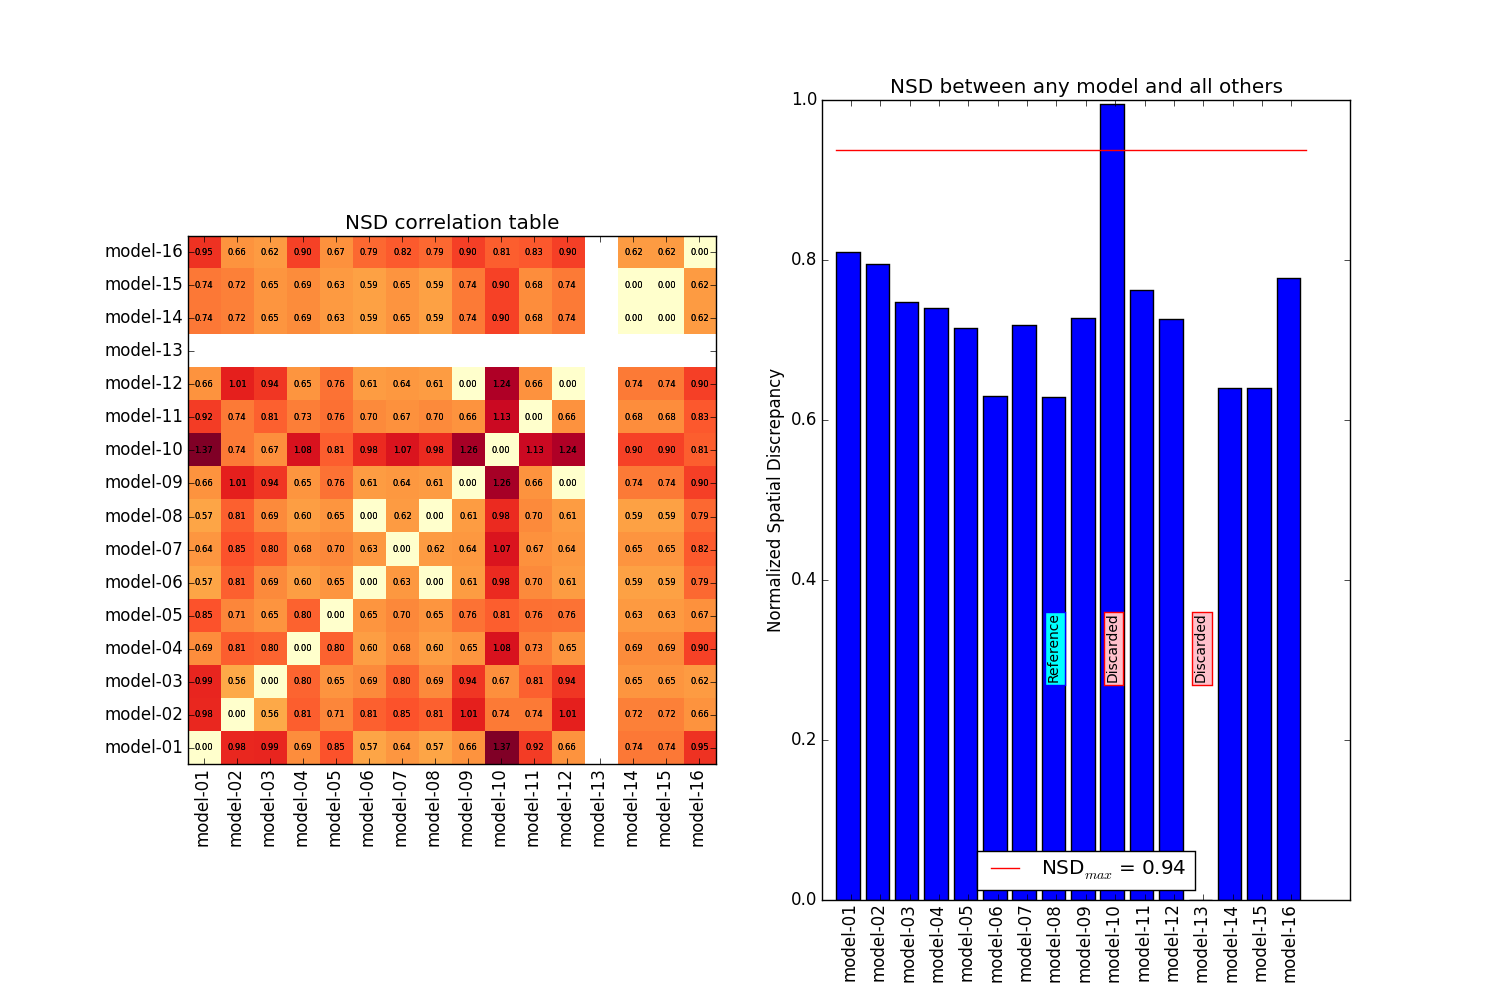
\includegraphics[width=8cm]{nsd.png}
\caption{Plots created by the pipeline for comparing a set of \textit{ab-initio} models.
The matrix on the left hand site gives the pair-wise normalized spatial discrepancy (NSD) between two models, using supycomb.
The bar plot on the right hand site gives the mean NSD.
The layout is adjusted from the standard version for improved readability in
print.}
\label{fgr:nsd}
\end{figure}

\begin{figure}
\centering
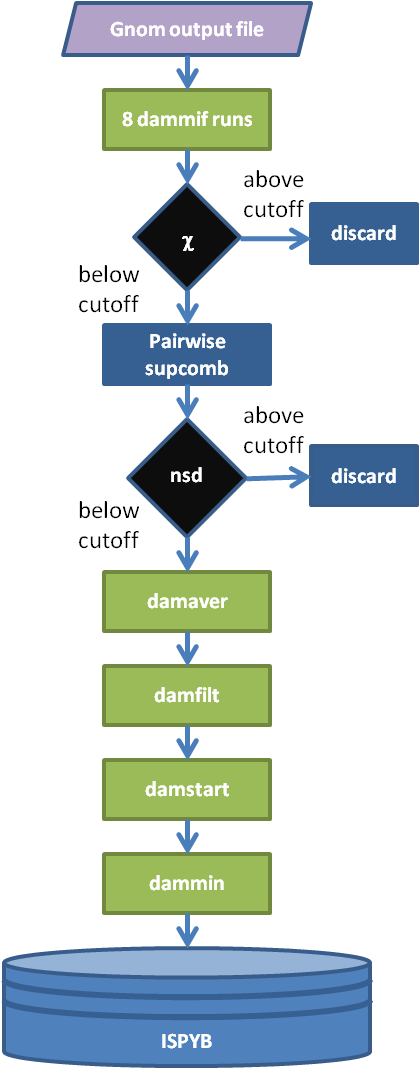
\includegraphics[width=8cm]{model.png}
\caption{Flow diagramm of the \textit{ab-initio} reconstruction plugin from a
\textit{gnom-file} (pair distance distribution function).
Symbols as described in figure \ref{fgr:smart}.}
\label{fgr:modeling}
\end{figure}

\begin{figure}
\centering
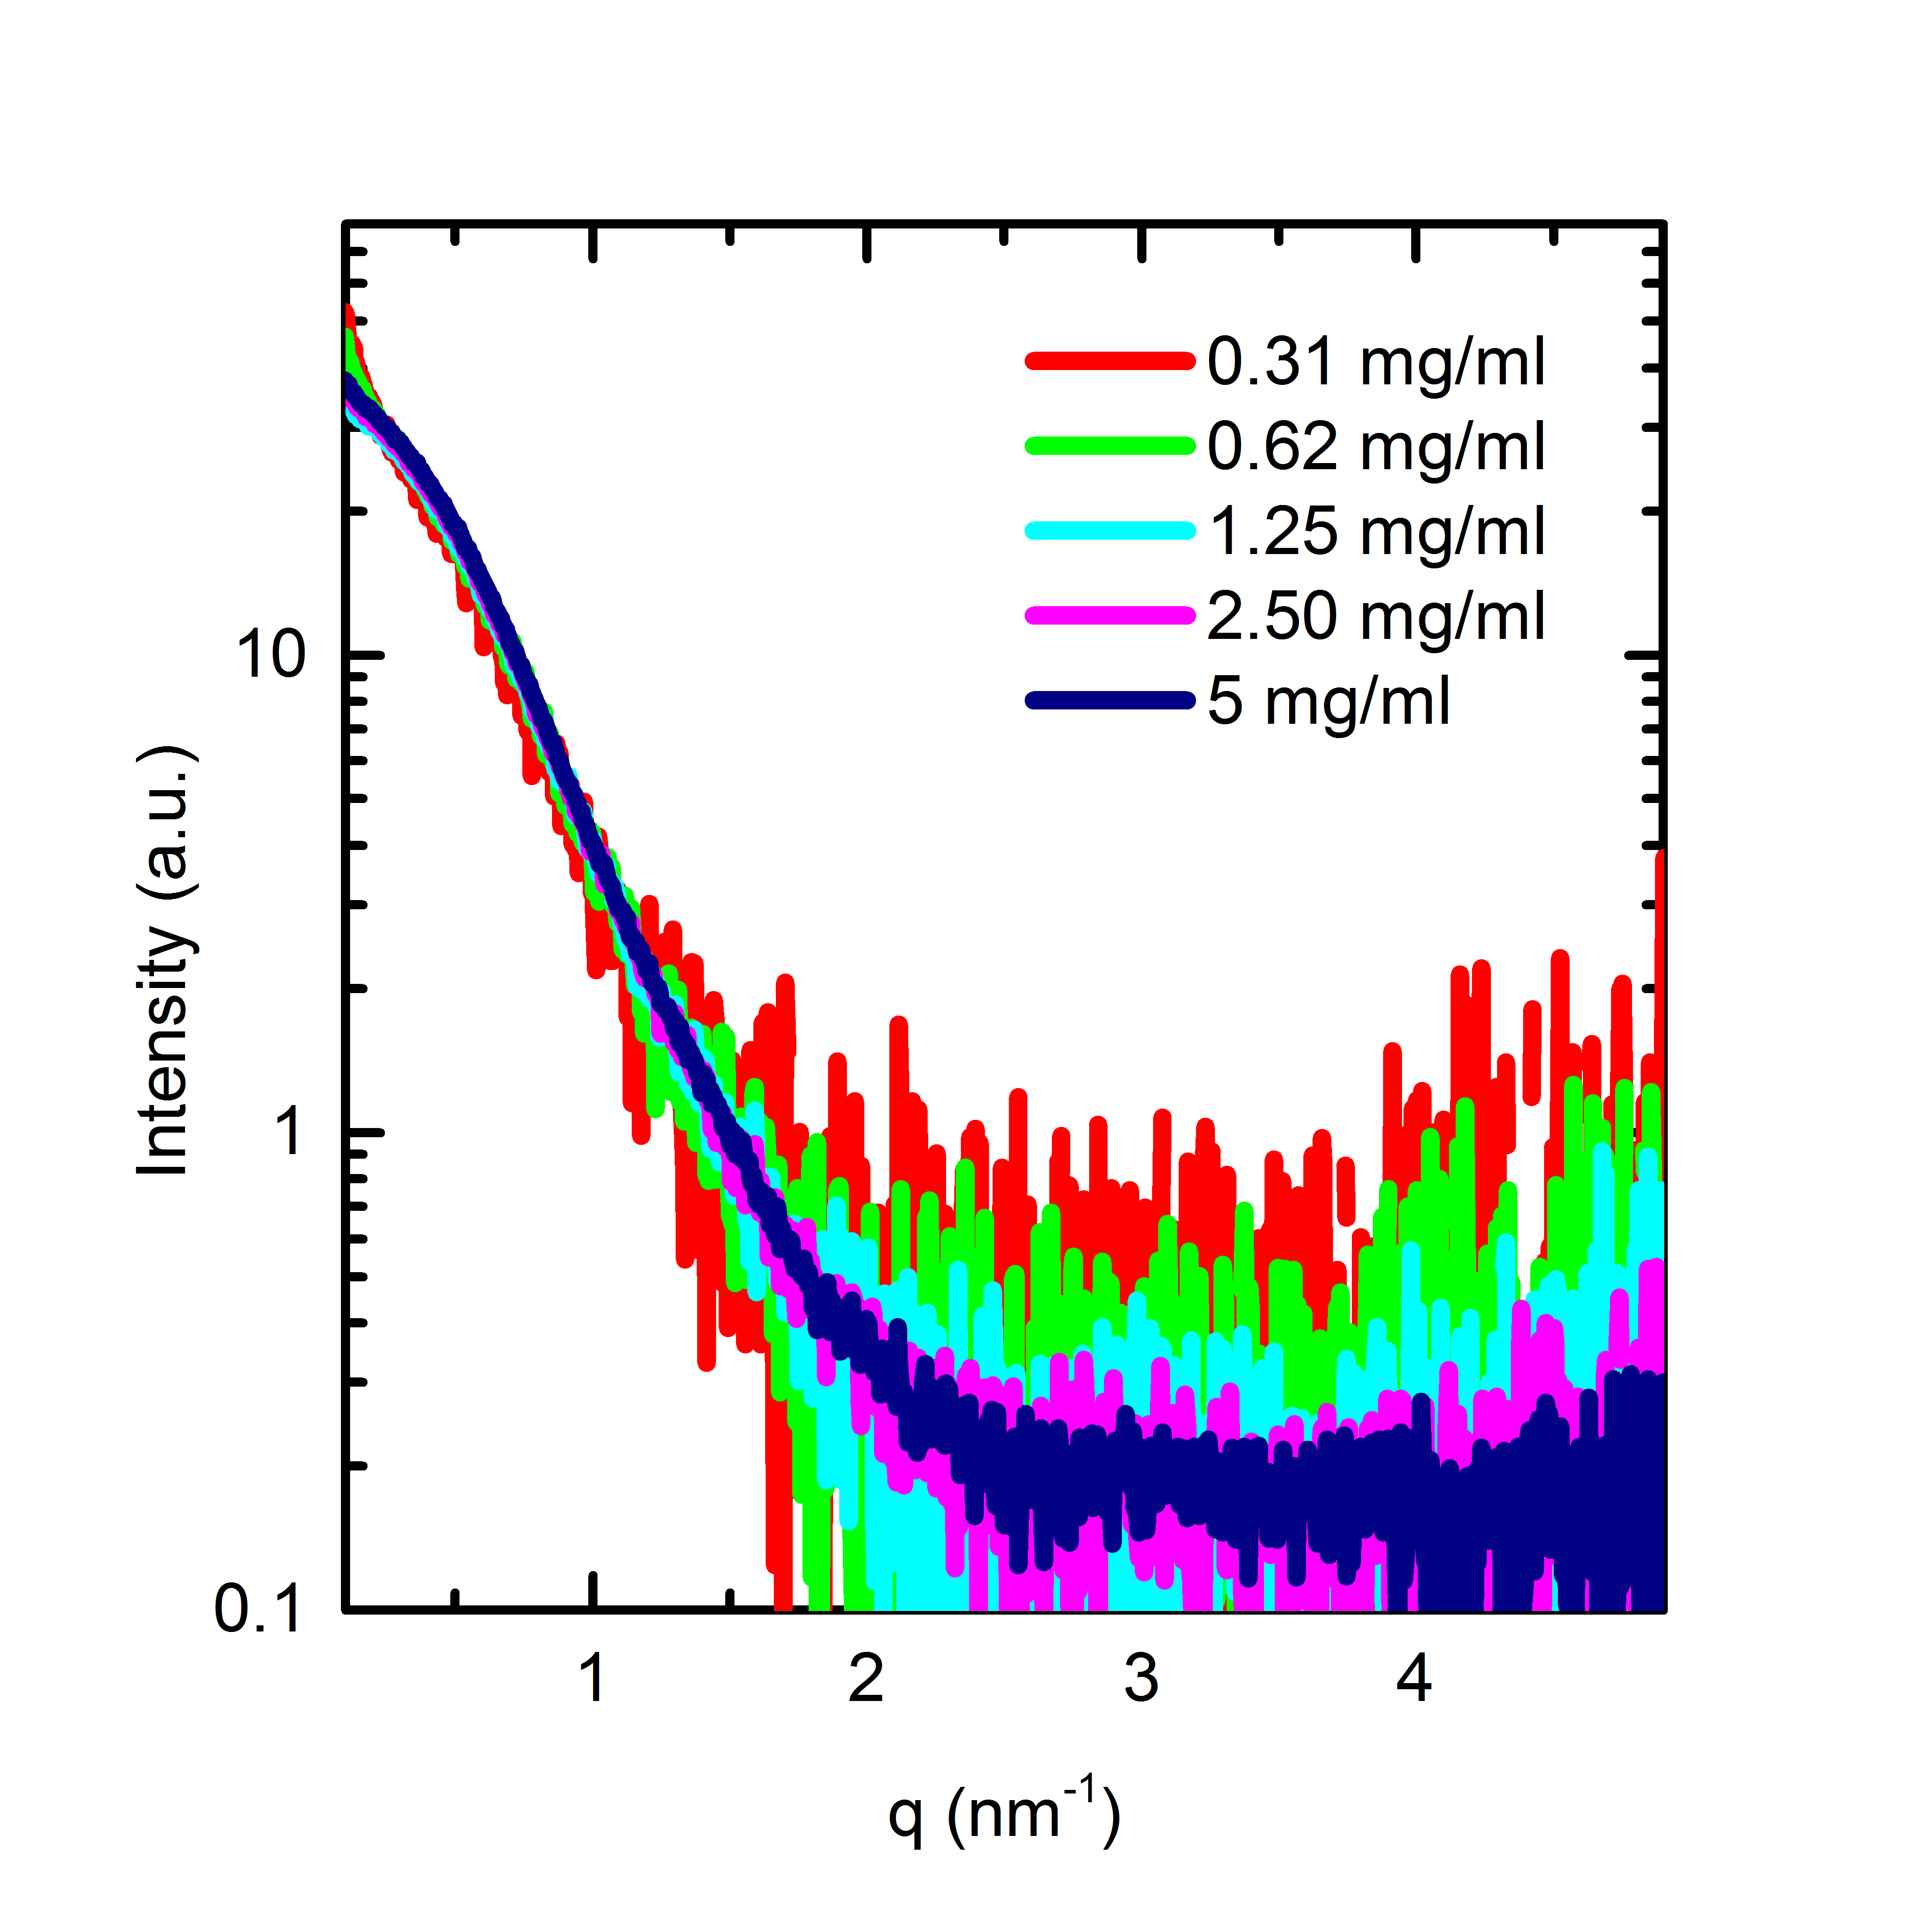
\includegraphics[width=8cm]{SCcurves.png}
\caption{Comparison of auto-subtracted SAXS curves of deletion construct of
protein D5 from vaccinia virus at different concentrations collected in SC mode.}
\label{fgr:SCcurves}
\end{figure}

\begin{figure}
\centering
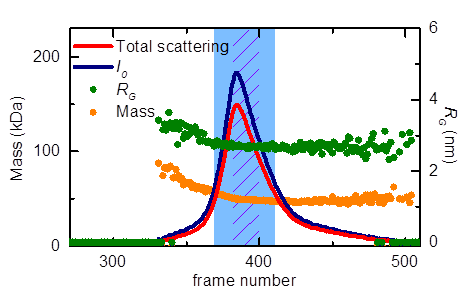
\includegraphics[width=8cm]{sec.png}
\caption{Chromatogramm of the SEC-SAXS experiment on the deletion construct of
protein D5.
The plot shows total scattering intensity ($\Sigma I$), forward scattering
($I_0$), radius of gyration ($R_G$) and estimated mass from the
auto-processing.
The region underlined in blue was used for automated merging of frames, the
striped region for manual merging.}
\label{fgr:SEC}
\end{figure}

\begin{figure}
\centering
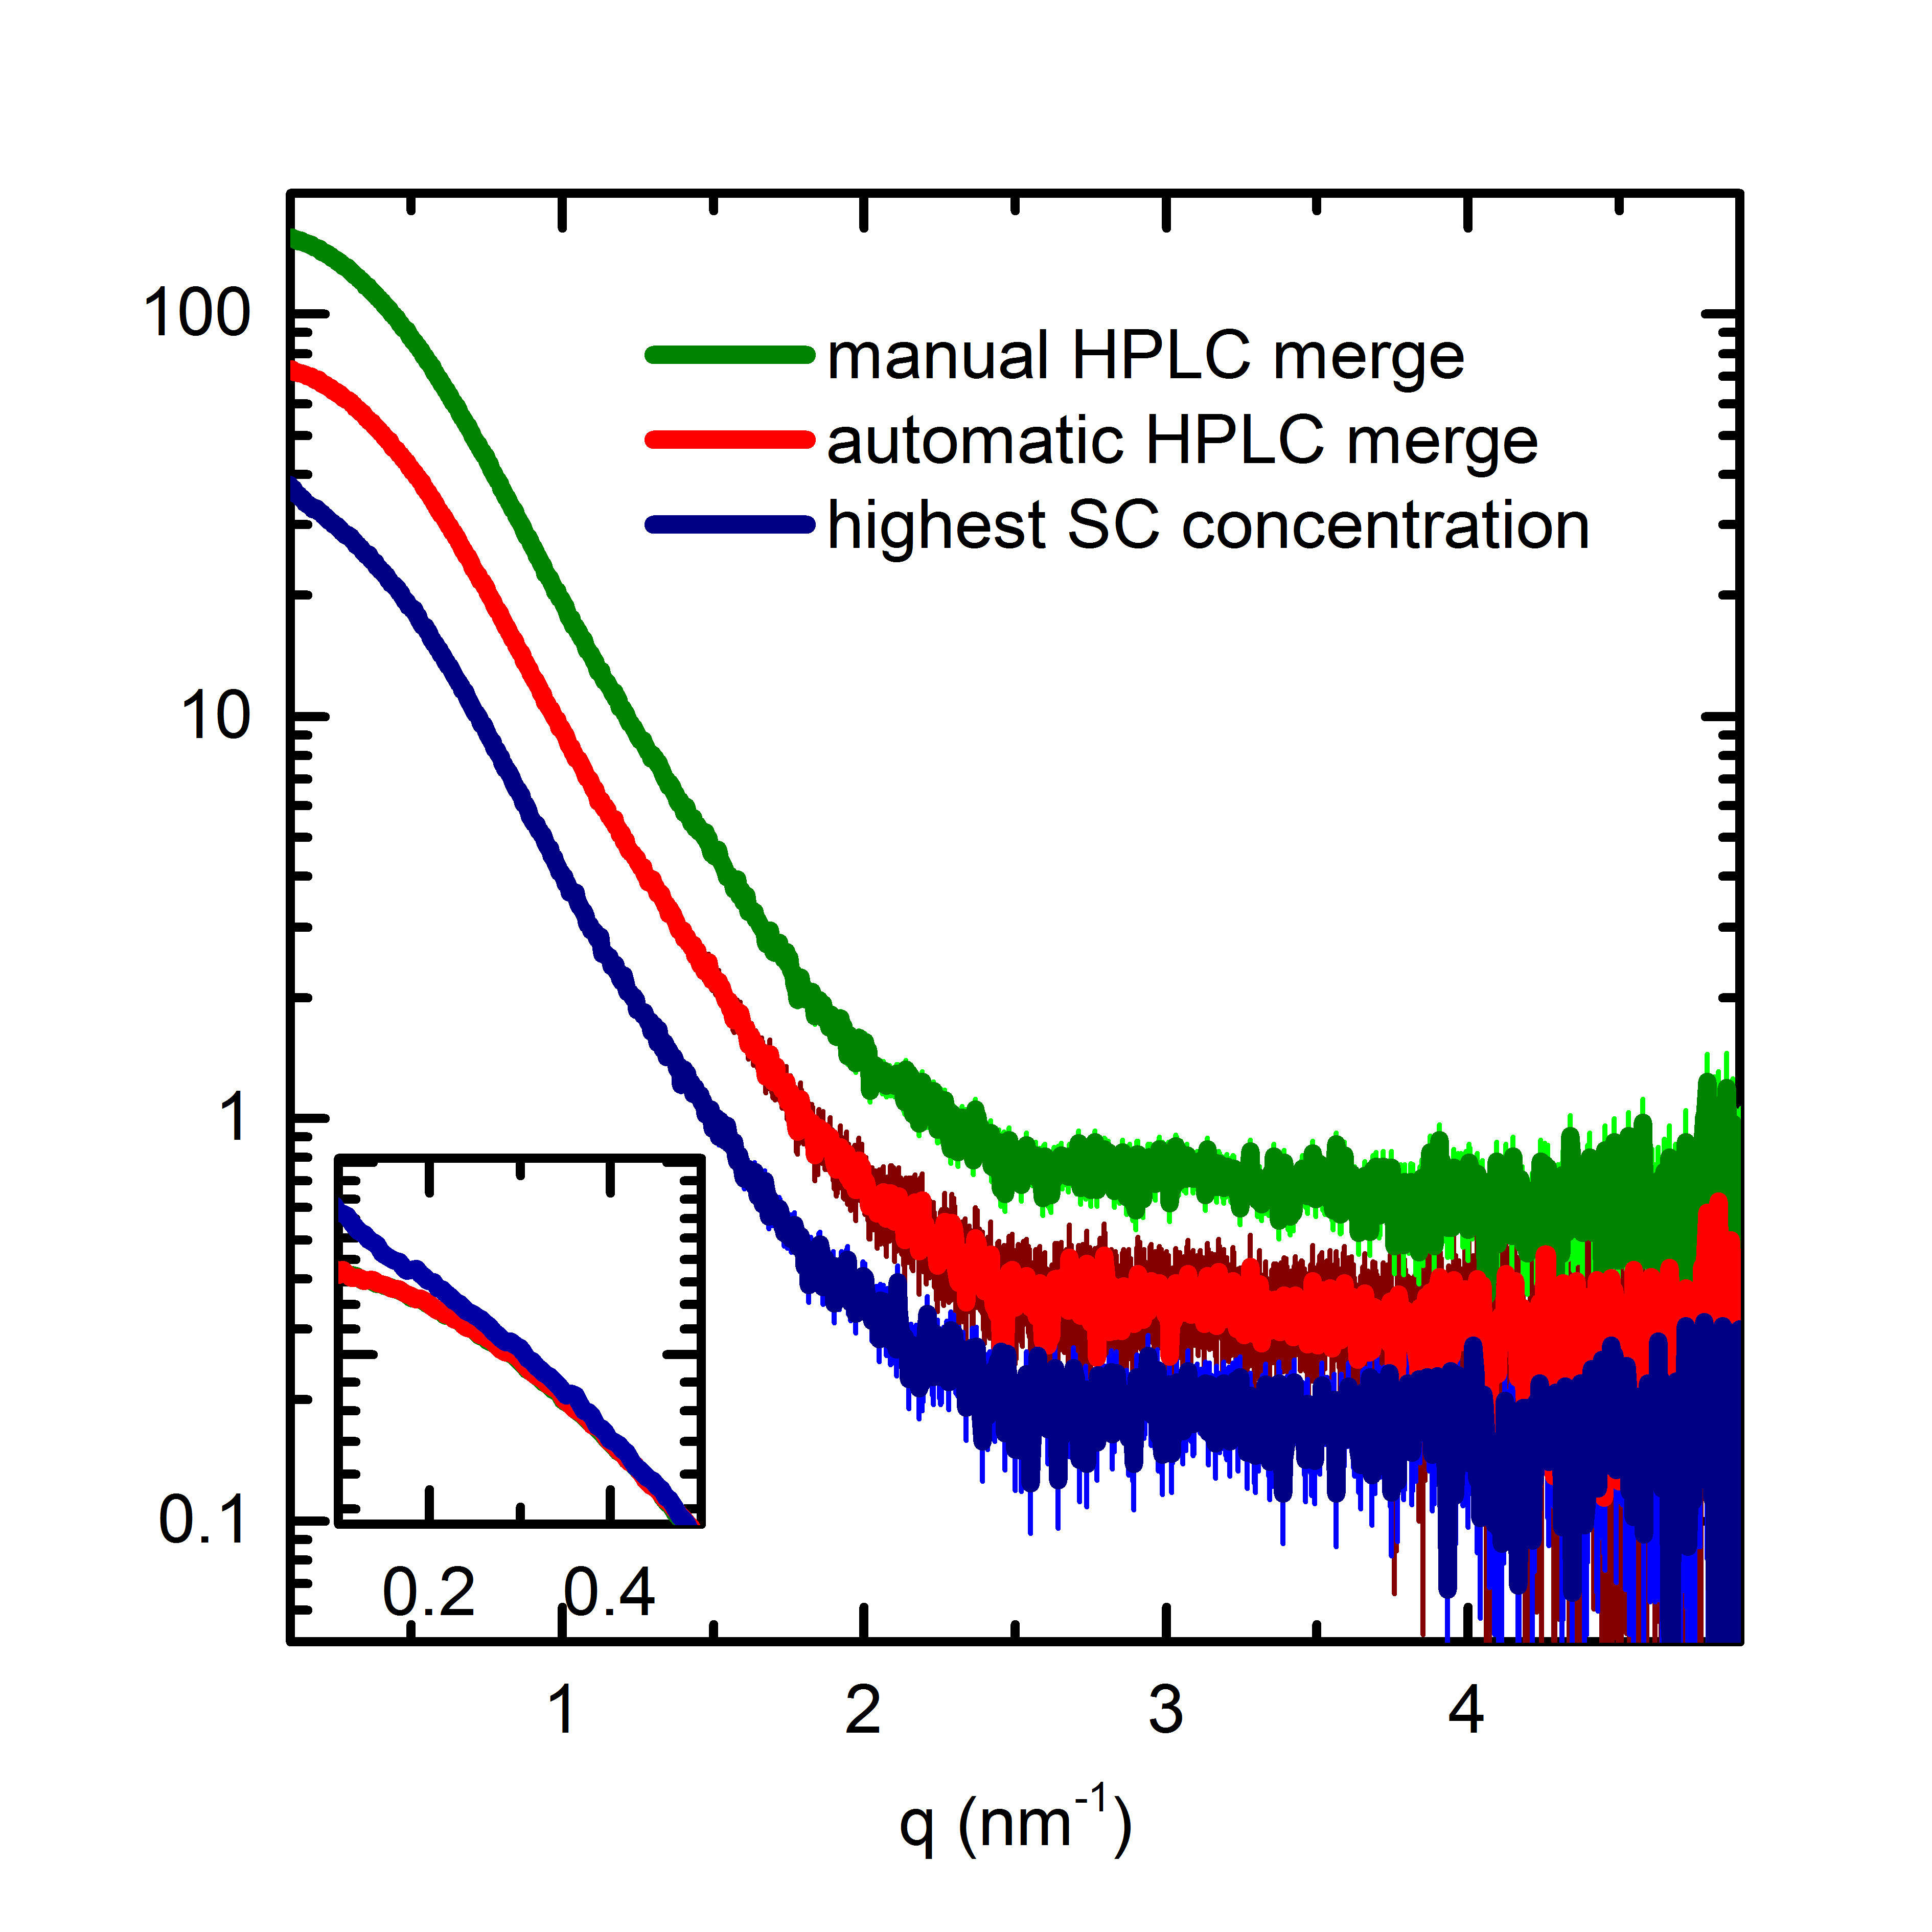
\includegraphics[width=8cm]{curves.png}
\caption{Comparison of subtracted curves: highest concentration collected in
sample changer mode (blue), automatic merge of SEC-SAXS data (red) and manual
merge of SEC-SAXS data (green). The inlay shows the differences between the SC
mode and SEC-SAXS data in the low-$q$ regime. }
\label{fgr:curves}
\end{figure}

\begin{table}
\begin{tabular}{ l c | c c c c c c }
   & $c$  & $I_{0}$  & $R_{G}$ & $D_{max}$ & $V_{P}$ & $V_{c}$ & Mass from $V_{c}$\\
	 &  (mg/ml) & (kDa) & (nm)&  (nm)&  (nm$^{3}$) & (nm$^{2}$) & (kDa)\\
\hline
Sample changer & 5.00  & 35.06 & 2.80 & 9.37  & 72.00 n& 4.18 & 50.85 \\
Sample changer & 2.50  & 34.28 & 2.83  & 9.91  & 72.08 & 4.20 & 50.15 \\
Sample changer & 1.25 & 33.58& 2.86  & 8.74  & 69.82 & 4.20 & 50.02 \\
Sample changer & 0.62  & 35.1& 2.99  & 10.48 & 73.89 & 4.40 & 52.73 \\
Sample changer & 0.31 & 35.83  & 3.26  & 8.72  & 74.42& 4.67 & 54.34 \\
HPLC, top of peak & - & 183.16 & 2.72  & -  & - & 4.08 & 49.70 \\
HPLC, merge & - & 123.89 & 2.70  & 9.46 & 69.97 & &  \\
Manual merge & - &  149.90 & 2.69 & 8.25 & & &  \\
\end{tabular}
\caption{Overview on the automatic processing results for the deletion construct of protein D5 from vaccinia virus. 
The expected mass of the protein is 45.5 kDa}
\label{tbl:results}
\end{table}


\end{document}
